% -*- mode: LaTeX; coding: utf-8; -*-

\documentclass[a4paper,12pt,titlepage]{article}

\usepackage{cmap}                   % правильный PDF (на первом месте)
\usepackage{ucs}                    % unicode
\usepackage[utf8x]{inputenc}
\usepackage{mathtext}               % перед загрузкой пакета babel
\usepackage[russian]{babel}
\usepackage{pscyr}                  % pretty cyrillic fonts
\usepackage{ifpdf}
\ifpdf
\usepackage[pdftex]{graphicx}       % pdf
\else
\usepackage{graphicx}               % dvips
\fi
\usepackage{indentfirst}            % правильный отступ
\usepackage{fancyhdr}               % нестандартные колонтитулы
\usepackage{floatflt}               % обтекание рисунков
\usepackage{lscape}                 % landscape (для таблицы)

\providecommand{\No}{\textnumero}   % fix obsolete \No
\graphicspath{{pictures/}}

%\renewcommand{\rmdefault}{ftm}

\ifpdf
\pdfinfo{
  /Author (Jan Musinsky)
  /Title (Detectors)
  /CreationDate (may 2007)
  /Subject (Detectors)
  %  /Keywords (Детекторы;Взаимодействие частиц с веществом)
}
\fi

\begin{document}
\title{\textcp{Газовые координатно-трековые детекторы}}
\author{\\ \LARGE{Ян Мушински} \\ \\
  ЛВЭ ОИЯИ Дубна \\ \\ \\}
% , Россия\\(университет и. Шафарика Кошице, Словакия
\date{\emph{май 2007 года}}
\maketitle

\thispagestyle{plain}
\setcounter{page}{2}
\tableofcontents

\clearpage
\pagestyle{fancy}
\fancyhf{} % clear all header and footer fields
\renewcommand{\sectionmark}[1]{%
  \markboth{#1}{}}
\fancyhead[R]{\slshape \leftmark}  % higher-level
%\fancyhead[R]{\slshape \rightmark} % lower-level
\fancyfoot[C]{\thepage}

% -*- mode: LaTeX; coding: utf-8; -*-

\thispagestyle{plain}
\section{Введение}
Изучение природы взаимодействия ядерной материи немыслимо без методов
регистрации частиц. Эти методы возникали и совершенствовались
по мере развития ускорительной техники, теоретических воззрений, увеличения
типов и энергии частиц и т.д. Во времена открытия лучей Рентгена
использовались обычные фотографические пластинки. Такие же "<детекторы">
способствовали открытию радиоактивности и сыграли важную роль в атомной
и ядерной физике.

Однако, по мере развития физики частиц, усложнялись требования к методам
наблюдения траекторий отдельных частиц, определению их природы. Это привело
к изобретению различного рода детекторов --- процессу, который продолжается
и по сей день. Появились камеры Вильсона, диффузионные и пузырьковые
камеры.

На первых порах эти приборы, а также специально изготовленные ядерные
фотоэмульсии использовались в наблюдении взаимодействий в космических лучах.
Эти редкие и беспорядочно направленные частицы из космоса создавали
трудности для регистрации их взаимодействий с веществом. Возникла проблема
сооружения "<космотронов"> --- так стали называть ускорители частиц высоких
энергий. Эти приборы развивались по своим законам. Физики стремились получить
всё более и более высокоэнергичные частицы.

Эксперименты на современных ускорителях требуют "<расшифровки"> сложных
событий, включающих сотни и тысячи вторичных частиц. Соответственно
усложнились и детекторы для их наблюдения и измерений параметров заряженных
частиц. Нашей задачей является сделать некоторый обзор средств наблюдения
вторичных частиц с акцентом на газовые координатно-трековые детекторы,
которые являются непременной составляющей всех экспериментальных установок.

Сначала рассматриваем физические процессы, происходящие при прохождении
частиц через вещество, которые позволяют регистрировать следы ионизирующих
частиц и без которых невозможно понять работу любого детектора. Затем
коротко останавливаемся на использовавшихся до последнего времени трековых
приборах различного типа с коротким анализом их преимуществ и недостатков.

Последний раздел реферата посвящён принципу работы наиболее широко
используемым в физических установках многопроволочным пропорциональным
и дрейфовым камерам.

\section{Взаимодействие частиц с веществом}
Принцип работы любого детектора связан с характером взаимодействия
частицы с веществом данного прибора. Заряженная частица или гамма квант,
проходящая  через материю, может потерять свою энергию частично или
полностью в зависимости от типа взаимодействия.

Если не считать очень слабого гравитационного взаимодействия, существуют
три вида взаимодействия излучения с веществом:
\begin{description}
\item[сильное (ядерное)] наиболее интенсивное. Оно может
проявляться как в процессах непосредственного взаимодействия, так и
в~процессах распада ядер или частиц. Сильные процессы характеризуются
очень большими сечениями и коротким действием сил.
\item[электромагнитное] второе по интенсивности. ~Определяет
взаимодействие заряженных частиц и $\gamma$-квантов. Дальнодействующий
характер сил и значительно большее число электронов в веществе, чем
атомных ядер, определяет доминирующую роль в процессе взаимодействия
излучения с атомами.
\item[слабое] кроме процессов распада, оно может проявляться и в
процессах захвата нейтрино (антинейтрино) нуклоном, однако сечение таких
процессов очень малое.
\end{description}

Главную роль при прохождении заряженных\footnote{Нейтроны
регистрируются по вторичным заряженным частицам, возникающим благодаря
их сильному взаимодействию с ядрами.}
%можно регистрировать косвенно, сначала они должны образовать вторичные
%заряженные частице благодаря сильному взаимодействию с ядрами.}
частиц и $\gamma$-квантов через вещество играют электромагнитные
взаимодействия. Правда, частицы могут взаимодействовать и с атомными
ядрами, однако основные потери энергии и эффекты рассеяния определяются
взаимодействием с атомными электронами. Поэтому интересующие нас
процессы скорее подчиняются атомной, а не ядерной физике.

По механизму прохождения через вещество частицы можно разделить
на следующие группы:
\begin{itemize}
\item[-] тяжёлые заряженные частицы ($p,~d,~\alpha$,~ ионы, \dots)
\item[-] лёгкие заряженные частицы ($e^\pm$)
\item[-] гамма---излучение
\item[-] нейтроны
\end{itemize}
\clearpage
Разные процессы взаимодействия частиц не позволяют нам рассматривать их
все вместе. Рассмотрим отдельно главные виды взаимодействий со средой
заряженных частиц (ионизационные потери, тормозное, черенковое излучение,
многократное рассеяние), $\gamma$-квантов (фотоэффект, Комптон эффект,
образование электрон---позитронных пар) и в~конце кратко обсудим
взаимодействие нейтронов с веществом.

\subsection{Ионизационные потери энергии}
Основные потери энергии быстрых тяжёлых заряженных частиц происходят 
в~результате кулоновского взаимодействия при столкновениях с~атомными
электронами. Заряженная частица либо возбуждает атом, либо ионизирует.
Такие процессы обычно называют ионизационными потерями или
торможением.

Средние потери энергии $-dE$ на единицу пути $dx$ для заряженных тяжёлых
$(m\gg m_e)$ частиц определяются формулой Бете---Блоха \cite{pdg}:
\[
-\frac{dE}{dx}=Kz^2\frac{Z}{A}\frac{1}{\beta^2}
\Biggl[\frac{1}{2}\ln\frac{2m_ec^2\beta^2\gamma^2T_{max}}{I^2}-\beta^2-\frac{\delta}{2}\Biggr],
\]
где
\begin{itemize}
\item $K=4\pi N_Ar_e^2m_ec^2$ = 0.307075 MeV/(g~cm$^{-2}$);
\item $z,~\beta = v/c$ - заряд и скорость налетающей частицы;
\item $Z, A$ - атомный номер и атомный вес среды;
\item $T_{max}$ - максимальная кинетическая энергия переданная электрону;
\item $I$ - средний ионизационный потенциал поглощающего вещества,
  приблизительно равный $I\cong 16~Z^{0.9}$ eV;
\item $\delta$ - параметр учитывающий релятивистский эффект поляризации
  среды пролетающей через неё релятивистской частицей (определяется
  экспериментально).
\end{itemize}
При анализе реальных экспериментов толщину вещества измеряют не
в~единицах длины, а величиной $\rho dx$, где $\rho$ плотность поглотителя.
Так называемые удельные потери энергии
$\frac{dE}{d(\rho x)}=\frac{1}{\rho}\frac{dE}{dx}$ принято приводить
в единицах $\frac{MeV}{g~cm^{-2}}$. Удельные ионизационные потери энергии
слабо зависят от свойств материала. На рис.~\ref{fig:loss1} хорошо виден
общий характер указанной зависимости.
\begin{figure}[h]\center
  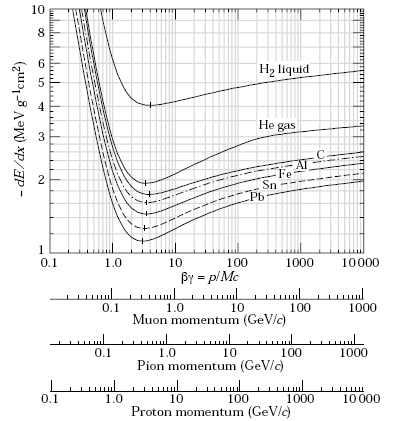
\includegraphics[scale=0.77]{loss1}
  \caption{Зависимость удельных потерь энергии в водороде, гелии,
    углероде, алюминии, железе, олове и свинце от импульса мюона,
    пиона и протона.}
  \label{fig:loss1}
\end{figure}

Формула приближенная, однако это приближение вполне достаточно (точность
порядка нескольких процентов). Уравнение несправедливо\footnote{
Добавляется параметр, который уменьшает ионизационные потери за счёт
связи электронов на K и L оболочках атомов.} для медленных частиц,
скорость которых сравнима со скоростями атомных электронов.
При этих скоростях потери энергии пропорциональны~$\beta$. С увеличением
скорости средние ионизационные потери приблизительно пропорциональные
$1/\beta^2$ и достигают достаточно широкого, так называемого,
ионизационного минимума $\beta\gamma\approx (3 \div 4)$ \cite{cer:04}.
%, так называемый ионизационный минимум.

При достаточно больших скоростях, когда $\beta$ приближается к~1,
множитель перед квадратной скобкой в~уравнение Бете---Блоха, перестаёт
изменятся. Зависимость потерь энергии от скорости частицы определяется
членами в~квадратных скобках: логарифмическим членом и
поправкой~$\delta$. Потери энергии снова начинают расти в соответствии
с возрастанием логарифмического члена (основная часть которого связана
с большими передачами энергии электронам, $\delta$-электроны).

При дальнейшем увеличении скорости возрастает влияние эффекта
поляризации среды. Электрическое поле пролетающей частицы
поляризует среду, и возникающие при этом экранирование останавливает рост
ионизационных потерь. Его часто называют эффектом плотности (зависимость
от концентрации электронов в веществе), и он более значителен для твёрдых
и жидких тел, чем для газов.

Заметим ещё, что ионизационные потери энергии не зависят от массы
частицы проходящей через вещество (при условие $m\gg m_e$), но
существенно зависят от её заряда и скорости (и концентрации электронов
в среде).

\subsection{Многократное рассеяние}
При прохождение через слой вещества заряженная частица испытывает
большое число взаимодействий. Преобладающим является кулоновское
рассеяние на малые углы. Многократное рассеяние описывает теория
Мольера. Иногда, частица рассеивается и на довольно
большие углы (столкновение заряженной частицы с ядром), но в соответствии
с формулой Резерфорда, вероятность с ростом угла, резко падает
$\frac{d\sigma}{d\Omega}\propto \frac{1}{\sin^4\theta /2}$.

Средний угол многократного кулоновского рассеяния даётся выражением
\cite{kor:06}:
\[
\theta_0=\frac{13.6~MeV}{\beta c p}~z~\sqrt{x/X_0}
\Big[1+0.038\ln(x/X_0)\Big],
\]
где $\beta c,~p,~z$ - скорость, импульс и заряд рассеянной частицы;
$x, X_0$ - толщина слоя среды и радиационная длина.
\begin{floatingfigure}[l]{5.7cm}
  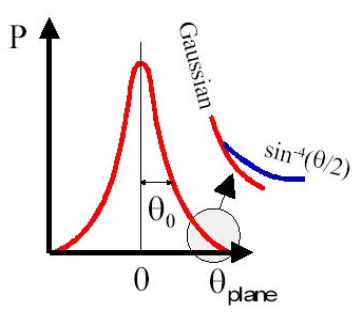
\includegraphics[width=5.0cm]{loss2}
\end{floatingfigure}
Распределение угла многократного рассеяния хорошо описывается гауссом.
При больших значениях угла, хвост распределения приближается к форме,
определённей формулой Резерфорда.

Для быстрой оценки радиационной длины можно использовать формулу:
\[
X_0\approx \frac{(716~g/cm^2)}{Z(Z+1)ln(287/\sqrt{Z})}\frac{A}{\rho},
\]
где $A, Z, \rho$ - атомный номер, атомный вес и плотность среды.

\subsection{Тормозное излучение}
\label{sec:breaking}
Заряженная частица которая движется с ускорением испускает
электромагнитное излучение, энергия которого пропорциональна квадрату
ускорения, а ускорение обратно пропорционально массе частицы. Для
тяжёлых частиц такие потери энергии ничтожно малы\footnote{Даже для
мюона, самой лёгкой частицы после электрона, радиационные потери 40.000
раз слабее, чем для электрона того же самого импульса \cite{kor:06}.},
другая ситуация в случае электрона. Быстрый электрон может тереть часть
энергии посредством испускания фотонов при торможении в электрическом
поле атомного ядра. Возникающие электромагнитное излучение называется
тормозным, а потери энергии частиц радиационными.

Соотношение между ионизационными и радиационными потерями энергии для
электронов можно оценить по формуле:
\[
\frac{(-\frac{dE}{dx})_{rad}}{(-\frac{dE}{dx})_{ion}} \approx \frac{E~Z}{800~MeV}
\]
Энергия при которой потери равны, называется критической, и для электронов
её можно определить из формулы $E_c \approx (800~MeV)/(Z+1.2)$ \cite{sta}.
\begin{figure}[h]\center
  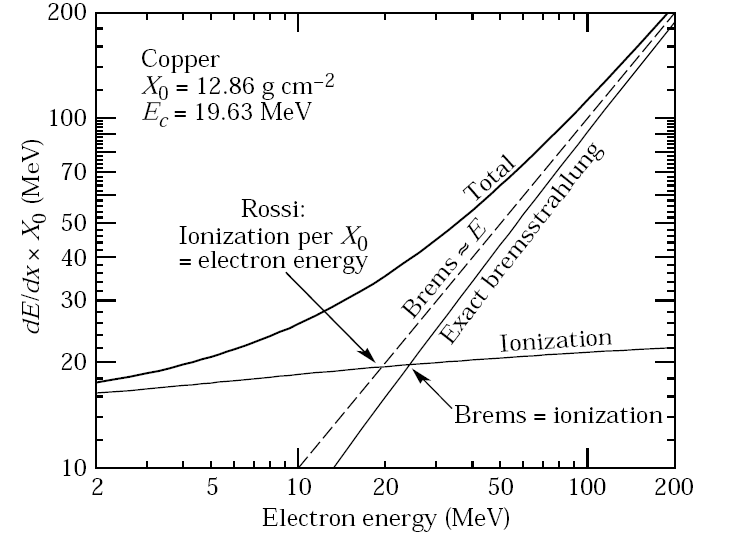
\includegraphics[scale=0.45]{loss3}
  \caption{Определение критической энергии $E_c$ электрона.}
  \label{fig:loss3}
\end{figure}

При больших энергиях электрона, когда ионизационными потерями можно
пренебречь, потери энергии на излучение можно выразить в виде:
\[
-\Bigg(\frac{dE}{dx}\Bigg)_{rad}=\frac{E}{X_0} \quad \Rightarrow \quad
E = E_0e^{-x/X_0},
\]
где $X_0$ - радиационная длинна, т.е. расстояние на котором энергия
в~результате потерь на излучение уменьшается в $e$ раз. Например, для
воздуха при нормальном давлении и температуре, радиационная длина
приблизительно 300 метров.

Видно, что высокоэнергетический электрон теряет свою энергию по
экспоненциальному закону. Однако многие фотоны испускаемые при
тормозном излучении имеют достаточную энергию для рождения
элек\-трон---позитронных пар, которые последовательно испускают фотоны
и т. д., таким образом, быстрые электроны создают так называемые
электромагнитные каскадные ливни (раздел~\ref{sec:showers}).

\subsection{Черенковское излучение}
\begin{floatingfigure}[l]{6.5cm}
  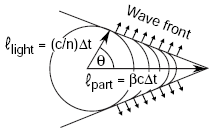
\includegraphics[width=6.0cm]{loss4}
\end{floatingfigure}
Заряженная частица, движущаяся со скоростью превышающей фазовую
скорость света в данной среде, испускает электромагнитное излучение,
называемое черенковским\footnote{излучение Вавилова---Черенка}.
Угол $\theta$ между направлением движения частицы и испускаемым
%электромагнитным %черенковским
излучением ровен $\theta =\arccos(1/n\beta)$, где $n$ - показатель
преломления вещества.
%$\cos\theta =\frac{1}{n\beta}$ где $n$ - показатель преломления среды.
%(только для $n>1$ частица может испускать данное излучение)

Этот эффект можно объяснить появлением поляризации атомов вдоль пути
движущейся частицы. Если она движется сравнительно медленно $v < c/n$,
возникающая поляризация будет распределена симметрично вокруг её пути.
Суммарное поле всех диполей равно нулю и излучения нет. Если скорость
частицы $v > c/n$, симметрия нарушается, образуется диполь и возникает
когерентное излучение.

Потери энергии на черенковское излучение учитываются формулой
Бете---Блоха (в области релятивистского возрастания), однако они
в~большинстве случаев составляют малую долю от общих потерь.
По сравнению с ионизационными потерями, их доля составляет несколько
процент. Для газов с $Z\geq7$ доля меньше чем 1\%, для лёгких газов
(He, H) приблизительно 5\% \cite{den:04}.

\subsection{Взаимодействие гамма---излучения}
Взаимодействие фотона с атомом среды приводит либо к полному поглощению
кванта, либо к существенному изменению направления его движения. Поток
фотонов с интенсивностью $I_0$ при прохождении через слой вещества
толщиной $x$ уменьшается по экспоненциальному закону:
\[
I(x)=I_{0}е^{-\mu x}.
\]
Массовый коэффициент поглощения $\mu$ связан с сечением различных
процессов взаимодействия фотонов $\sigma_i$ выражением
$\mu=\frac{N_A\rho}{A}\sum\sigma_i$, где $N_A$~-~число Авогадро,
$A$ - атомный вес и $\rho$ - плотность вещества. Сечение поглощения
$\gamma$-квантов сильно зависит от энергии фотона и представляет суммарный
вклад всех механизмов взаимодействия фотонов с веществом,
рис. \ref{fig:loss5}.
\begin{figure}[h]\center
  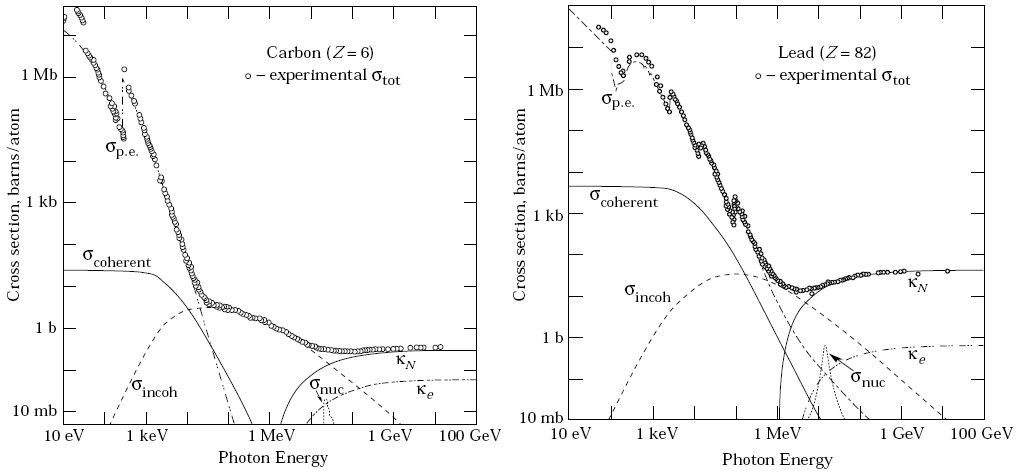
\includegraphics[scale=0.45]{loss5}
  \caption{Сечение полного поглощения фотонов с углеродом и свинцом.}
  \label{fig:loss5}
\end{figure}

Основный вклад в поглощение при низких энергиях ($E_\gamma$ < 0.1 MeV)
даёт фотоэффект, при средних энергиях (0.1 MeV < $E_\gamma$ < 10 MeV)
эффект Комптона, а~при высоких энергиях ($E_\gamma$ > 10 MeV)
преобладает процесс образования электрон---позитронных пар \cite{mas:06}.
\paragraph{Фотоэффект} процесс взаимодействия $\gamma$-кванта с связанным
электроном. Атомный электрон полностью поглощает энергию фотона, при
этом вырывается из атома. Основный вклад (80\% из полного сечение
фотоэффекта) даёт сечение на K-оболочке атома. Вероятность фотоэффекта
резко зависит от заряда атома $Z$ и энергии фотона
$\varepsilon=E_\gamma/(m_ec^2)$
\[
\sigma_{ph}\propto\frac{Z^5}{\varepsilon^3}.
\]
\paragraph{Комптон---эффект} или комптоновское рассеяние. Это рассеяние
$\gamma$-кванта на свободном электроне\footnote{Когерентное рассеяние
фотонов на атоме как целом называется рэлеевским рассеянием. При этом
частота излучения до и после взаимодействия остаётся неизменной.}.
Если энергия фотона существенно превышает энергию связи электрона
в атоме, можно считать электрон квазисвободным (энергией связи
пренебрегается). Энергию рассеянного фотона приобретает электрон отдачи.
Сечение комптоновского рассеяния имеет приблизительно вид
% зависит от энергии фотона и возрастает в $Z$ раз
\[
\sigma_{C}\propto Z~\frac{\ln\varepsilon}{\varepsilon}.
\]
\paragraph{Образование пар} процесс рождения электрона и
позитрона при взаимодействии $\gamma$-кванта с кулоновским полем
атомного ядра. Энергия фотона полностью передаётся образовавшимся
электрону и позитрону, а также ядру, которое получает отдачу. Однако
энергия отдачи, передаваемая ядру, обычно столь мала, что ею можно
пренебречь. Таким образом пороговая энергия образования
электрон---позитронных пар в~поле ядра\footnote{Заметим также, что
образование $e^- e^+$ пар происходит и в кулоновским поле электрона, но
оно сильно подавлено по сравнению с рождением пар в поле ядра.}
определяется как $E_{pair}\approx2m_ec^2$. При больших энергиях, сечение
становиться практически независимым от энергии $\gamma$-кванта, а
определяется лишь зарядом атома
\[
\sigma_{pair}\propto Z^2\ln\frac{183}{Z^{1/3}}.
\]

\subsection{Электронно---фотонные ливни}
\label{sec:showers}
Преобладающим процессом взаимодействия высокоэнергичных электронов
является тормозное излучение (раздел~\ref{sec:breaking}).
Испускаемые фотоны высоких энергии, рождают электрон---позитронные
пары.
\begin{figure}[h]\center
  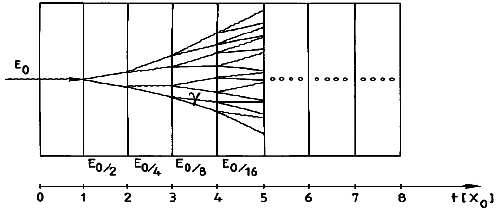
\includegraphics[height=4.4cm]{loss6}
  % \caption{Схематическое развитие электромагнитного ливня.}
  % \label{fig:loss6}
\end{figure}
Это в результате приводит к возникновению электрон---фотонных
ливней. Направление потока частиц, которые возникают, практически
совпадает с направлением первичной частицы.
%Модель развитие такого ливня показано на рис.~\ref{fig:loss6}.

Поток частиц ливня после своего образования сначала резко увеличивается.
Число частиц в ливне (сумма электронов, позитронов и фотонов) на глубине
$t$ составляет $N(t)=2^t$, где $t=x/X_0$ в единицах радиационной длины,
и энергия частицы на данной глубине равна $E(t)=E_0/2^t$. Максимальное
число частиц при развитии ливня достигается на глубине
$t_{max}=\frac{\ln E_0/E_c}{\ln2}$ и в максимуме составляет
$N_{max}\approx E_0/E_c$.

Когда энергия частиц ливня уменьшается настолько, что ионизационные
потери начинают преобладают над радиационными, ливень прекращается.
Значение энергии, когда она становится критической, можно выразить
как $E_c=E_0/2^{t_{max}}$ \cite{kor:06}.

Отмеченные закономерности существенны при конструкции калориметров,
которые можно использовать при измерении энергии электронов и фотонов
в экспериментах с частицами высоких энергии.

\subsection{Взаимодействие нейтронов с веществом}
Нейтроны взаимодействуют с веществом в основном за счёт их взаимодействия
с атомными ядрами посредством ядерных сил\footnote{Сечение
электромагнитного взаимодействия нейтрона, эффект от взаимодействия
магнитных моментов нейтрона и атомного электрона, приблизительно
в~$10^6$ раз меньше, чем для электрона (за исключением, когда эффект
происходит в ферромагнетиках).}. Поэтому регистрация нейтронов связана
с взаимодействием при котором сначала должны образоваться ионизирующие
частице.
\begin{floatingfigure}[l]{3.9cm}
  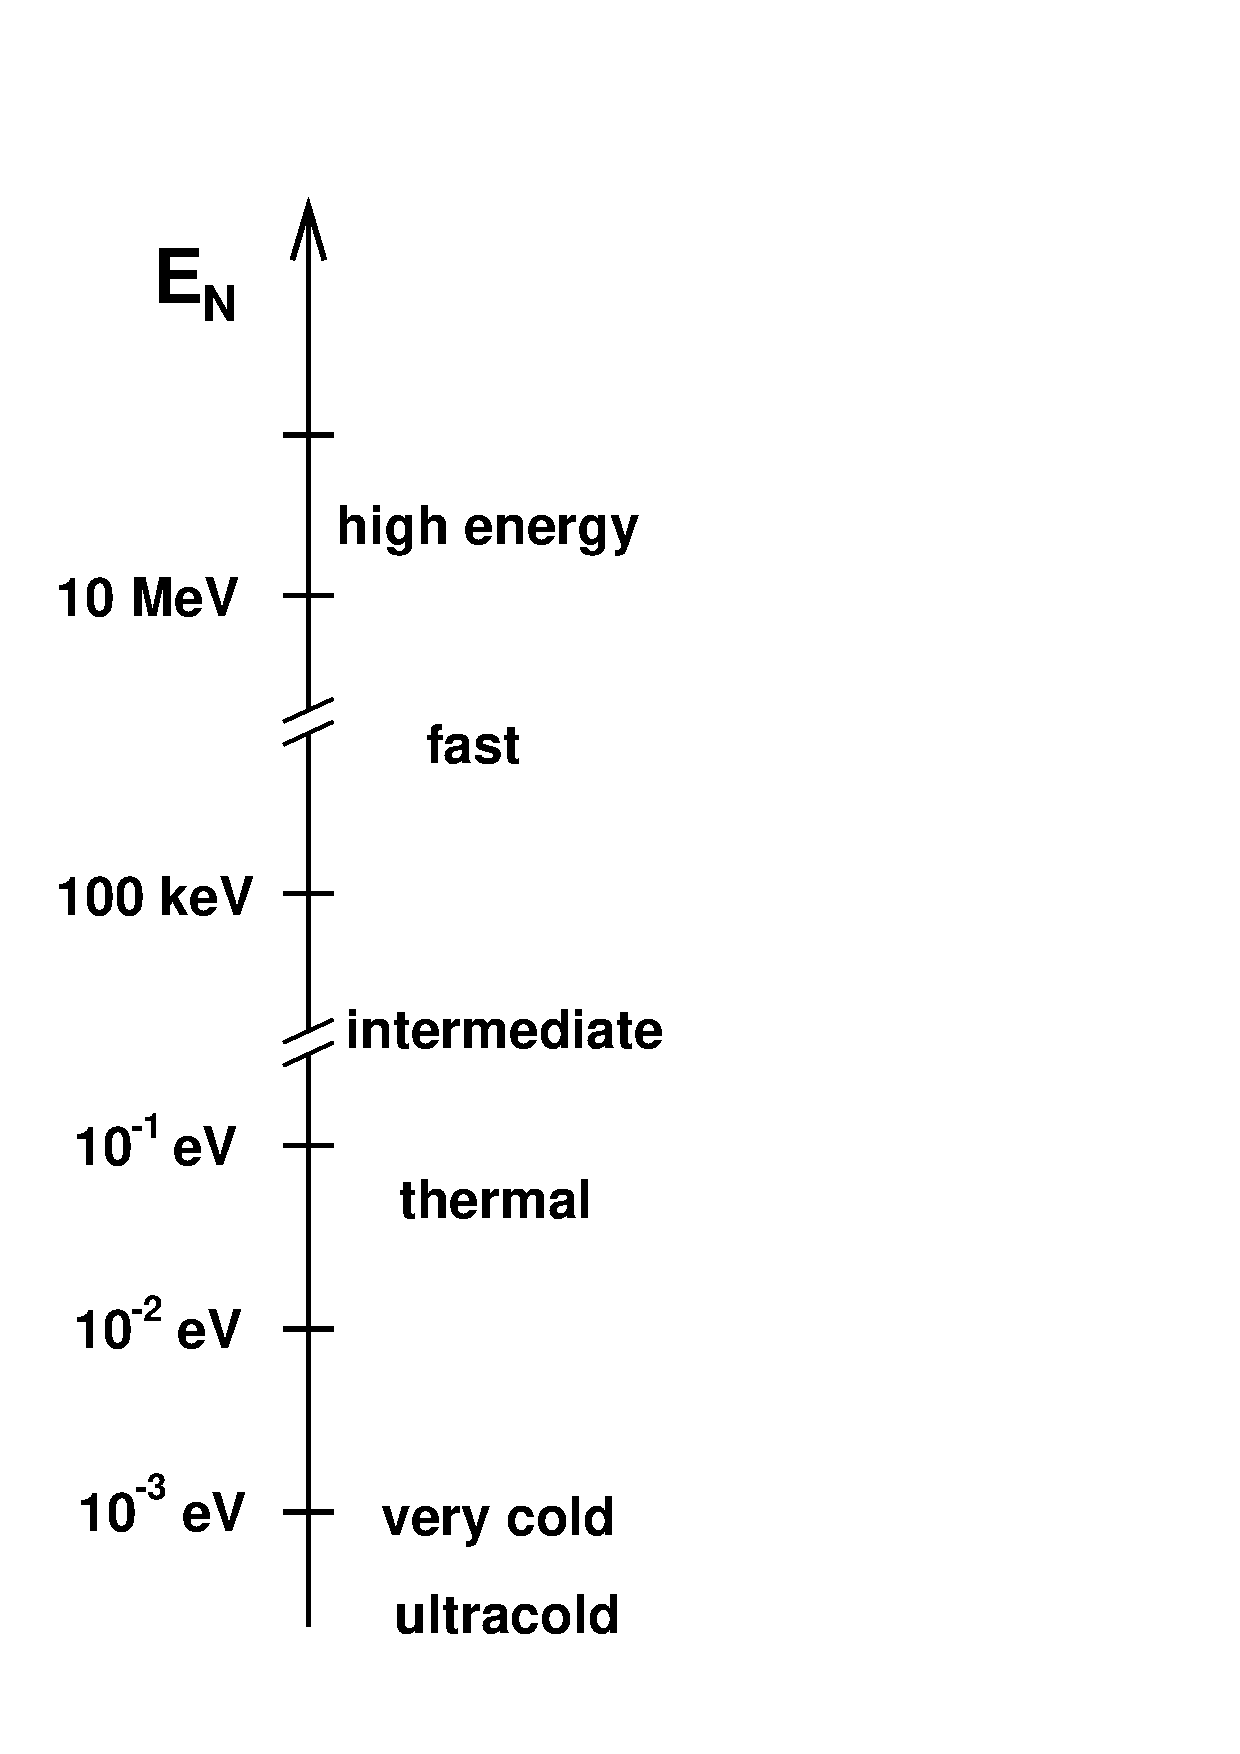
\includegraphics[width=3.1cm]{loss7}
\end{floatingfigure}
\hspace{-0.3cm}
Сечение взаимодействие нейтронов с веществом сильно зависит от энергии
нейтрона. Условно принято называть нейтроны с энергиями в интервале
от 0 до 100 keV, медленными. Если энергия выше, это быстрые нейтроны.
Медленные нейтроны ещё принято разделить на несколько интервалов:
ультрахолодные (самые низко энергичные), холодные, тепловые  и так
называемые промежуточные. Для нейтронов того или иного энергетического
интервала, следует применять разные методы регистрации \cite{kal:66}.

В зависимости от того, попадает нейтрон в ядро или нет, можно разделить
его взаимодействие с ядром на две группы: \clearpage
\paragraph{упругое рассеяние} без проникновения частицы
в~ядро (потенциальное рассеяние на силовом поле ядра). Ядро отдачи
приобретает кинетическую энергию и сможет ионизировать в~среде.
\paragraph{разнообразные ядерные реакции:} радиационный захват
(n, $\gamma$), реакции с~образованием одной или нескольких частиц (n, p),
(n, $\alpha$), неупругое рассеяние, упругое рассеяние при котором нейтрон
заходит в~ядро (резонансное рассеяние), деление ядер и т. п. Как правило,
эти реакции сопровождаются вылетом из ядра быстрых заряженных частиц,
которые могут в~веществе создать ионизационные эффекты.
\vspace{5.0cm}
\begin{figure}[h]\center
  \hspace*{-0.5cm}
  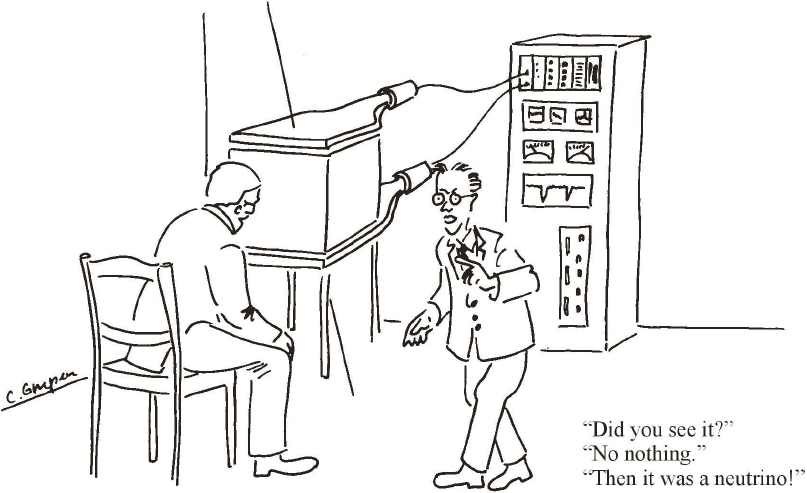
\includegraphics[width=15.0cm]{loss_last}
\end{figure}



%%% Local Variables:
%%% TeX-master: "referat"
%%% End:


\setcounter{footnote}{0}
% -*- mode: LaTeX; coding: utf-8; -*-

\section{Трековые детекторы}
Детекторы --- приборы для регистрации и локализации излучения. Если,
кроме самого факта и момента попадания частицы в объём
детектора\footnote{Такие детекторы обычно называют счётчиками.}, частица
оставляет след, это так называемые трековые детекторы. Они позволяют
существенно увеличивать информацию о происходящем процессе.

Основные характеристики детекторов, которые будут в дальнейшем
упоминаться:
\begin{description}
\item[\it временное разрешение]--- минимальный период времени, между
  двумя прошедшими частицами, когда сигналы не накладываются друг на
  друга. Если окажется, что в течение этого времени через детектор пройдёт
  больше чем одна частица, то он может регистрировать их как одну
  частицу.
\item[\it пространственное разрешение]--- аналогично с предыдущим.
  Характеризует погрешность, с которой детектор может различать положение
  частиц в пространстве.
\item[\it мёртвое время]--- время восстановления, которое должно пройти
  с момента регистрации одной частицы до момента, когда детектор снова
  сможет регистрировать следующую частицу. Если частица попадает
  в детектор за это время, то она не регистрируется.
\item[\it эффективность]--- вероятность того, что частица, пролетевшая
  через объём детектора будет зарегистрирована. Её можно определить как
  отношение числа зарегистрированных частиц, к числу всех прошедших
  через него частиц.
\end{description}
К главным представителям трековых детекторов относятся камера Вильсона,
пузырьковая камера, искровая камера, пропорциональные и дрейфовые
камеры. В таблице, в конце реферата, приведены все их основные
характеристики.

\subsection{Камера Вильсона}
Старейшим трековым детектором является камера Вильсона. Её изобретатель
в~1912 году установил, что пересыщенный пар конденсируется и образуют
видимые капли жидкости вдоль пути пролетающей через камеру заряженной
(ионизирующей) частицы. Обычно рабочей средой камеры являлась смесь из
паров воды и спирта. Пересыщение создаётся адиабатическим расширением
газа. Приблизительно за сотую долю секунды капли вырастают до больших,
видимых размеров. Трек, который создала заряженная частица в виде следов
из капелек, фотографируется. После этого газ в камера снова сжимается,
капельки испаряются. Электрическое поле очищает рабочий объём от
оставшихся ионов.
\begin{floatingfigure}[r]{7.2cm}
  \hspace{-0.5cm}
  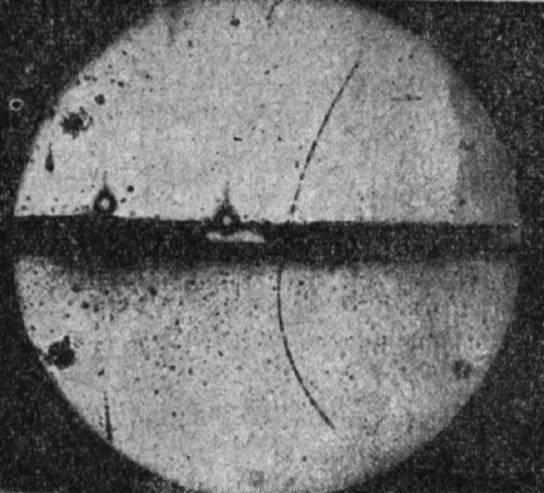
\includegraphics[width=7.0cm]{det01}
\end{floatingfigure}
Камера Вильсона сыграла выдающую роль в ядерной физике и физике
космических лучей. Ч.~Вильсон получил в~1927~г. Нобелевскую премию.
С~её помощью был, например, в~1932 году Андерсоном обнаружен позитрон
в космических лучах.
На протяжении нескольких десятилетий она была практически единственным
\footnote{В 40-е годы начались использоваться тоже ядерные эмульсии,
  которые применяются в экспериментах до сегодняшнего дня.} трековым
детектором. В~начале второй половины двадцатого века ей на замену
пришла пузырьковая камера.

\subsection{Пузырьковая камера}
Пузырьковая камера была изобретена Глэзером в 1952 году. Камера наполнена
перегретой жидкостью. Такая жидкость (обычно это жидкий водород)
неустойчива, и поэтому пролетающая через неё ионизирующая частица,
заставляет её мгновенно вскипать, вдоль пути частицы появляется цепочка
пузырьков пара. Перегретое состояние жидкости достигается резким
уменьшением давления. Камера становится на несколько миллисекунд
чувствительной (желательно это время синхронизовать со~временем
вхождения в камеру частиц из ускорителя). Образовавшийся, из цепочки
пузырьков пара, трек освещается и фотографируется. Заполняющая объём
жидкость, является одновременно и детектором и мишенью, это даёт
хорошую возможность получить почти полную картину взаимодействия.

Д. Глэзер в 1960 году получил за её изобретение Нобелевскую премию.
Развитие камер шло быстрыми темпами. В 70-х годов прошлого века они были
основными детекторами в физике высоких энергии. Рост энергий пучков
потребовал разработки камер огромных размеров.
Рабо- \newpage \noindent чий объём пузырьковых камер возрос почти
в миллионы раз \cite{har}.
\begin{figure}[h]\center
  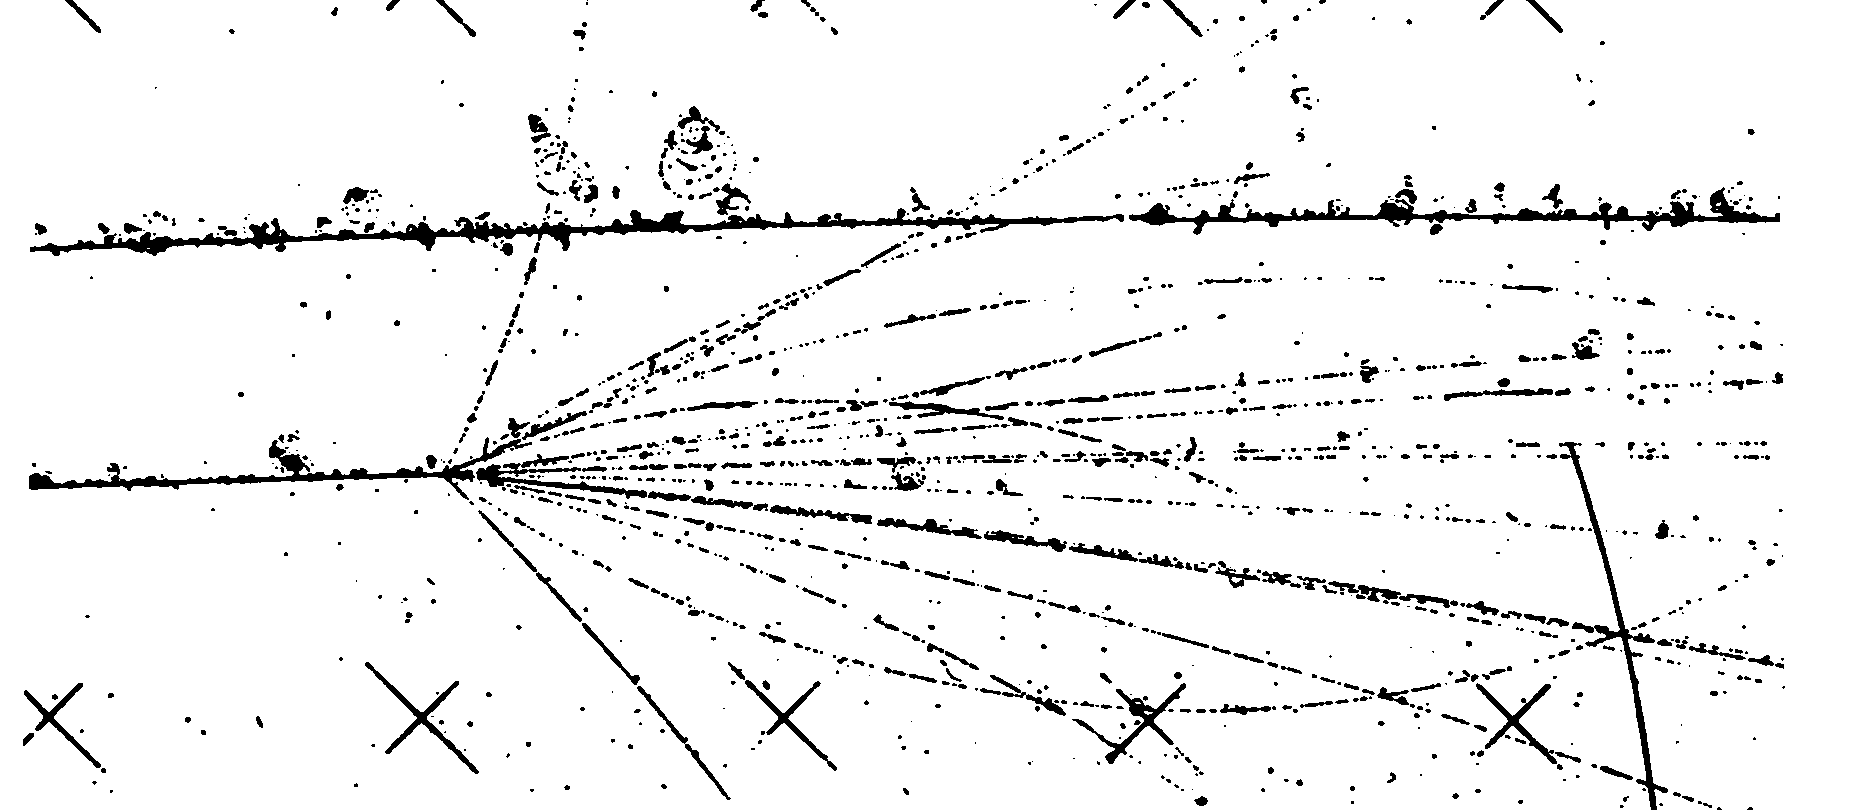
\includegraphics[scale=0.82]{det02}
  \caption{Полная дезинтеграция ядра фтора в водородной камере. Снимок из
    последнего сеанса 100-см водородной пузырьковой камеры ЛВЭ ОИЯИ
    в ноябре 1992 года \cite{gla}.}
\end{figure}

Несмотря на трудоёмкую работу связанную с расшифровкой фотографий
(восстановлением треков), основной недостаток пузырьковой
каме\-ры --- невозможность в процессе облучения выбрать интересующие нас
события, что приводит к необходимости просмотра большого количества
снимков.

\subsection{Искровая камера}
\begin{floatingfigure}[r]{0.20\textwidth}
  \vspace{-0.5cm}
  \hspace{-0.6cm}
  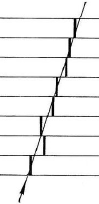
\includegraphics[width=0.18\textwidth]{det03}
\end{floatingfigure}
В конце 50-х годов прошлого века, появилась искровая камера. Она обычно
состоит из нескольких параллельных, плоских металлических пластин, которые
используются в качестве электродов. Пространство между ними заполняется
газом, чаше всего используется неон, гелий или аргон. Заряженная частица,
проходящая через камеру, образует ионы в газе. Одновременно (или
с маленьким опозданием $\sim$1 мкс), по сигналу совпадения из логического
устройства, обычно пара сцинтилляционных счётчиков, на электроды подаётся
короткий ($\sim$10-100 нс), высоковольтный ($\sim$10-20кВ/см) импульс
напряжения \cite{duk:04}. В~результате в месте прохождения частицы за
несколько наносекунд происходит видимый глазом искровой разряд\footnote{
  В стримерной камере, аналоге искровой камеры, формируются короткие
  светящиеся области, так называемые стримеры.}.
Возникающие искровые каналы фотографируются.

Искровая камера была хорошим дополнением к пузырьковой камере.
Появилась возможность управляемого запуска с помощью триггерных
счётчиков, для регистрации только нужных событий. Кроме того искровая
камера была способна работать более чем в сто раз чаще чем пузырьковая,
а~если время пролёта между частицами больше чем мёртвое время (время до
полного удаления заряда, образовавшего искры, оно приблизительно
несколько миллисекунд), то эффективность приближается к~100$\%$.

% Развитие, в это время вычислительной техники, позволило осуществить
% первые попытки замени оптической, фильмовой методики на электронный
% сбор данных.

\vspace{0.6cm}
\subsection{Ядерные фотоэмульсии}
Трек заряженной частицы можно регистрировать и методом аналогичным
обычному фотографированию. За развитие такого метода и открытия,
связанные с мезонами, сделанные с помощью фотографического метода
Ф.~Пауэлл в~1950~г. получил Нобелевскую премию.
\begin{floatingfigure}[r]{5.0cm}
  \hspace{-0.6cm}
  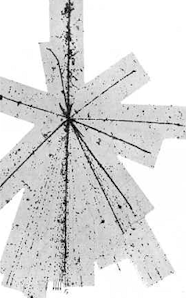
\includegraphics[width=4.8cm]{det04}
\end{floatingfigure}
Пластинки ядерных эмульсий состоят из мелких (0.2 $\div$ 0.3 мкм)
кристаллов бромида серебра, помещённых в слоях желатины \cite{nak:06}.
Отдельные слои складываются в стопку нужного объёма, обычно порядка
десятков сантиметров. Заряженная частица, проходящая через слои эмульсии,
вызывает химическое изменение в зёрнах бромида серебра, расположенных
вдоль трека ионизирующей частицы. Образуются зёрна металлического
серебра. Оставленный след в~фотоэмульсии просматривается микроскопом.
Отсюда и следует главный недостаток метода, очень трудоёмкая обработка
каждого слоя.

Однако, этот один из старейший методов регистрации частиц используется
до сих пор. В последнее время вновь возродилась техника фотоэмульсии.
Проводятся гибридные эксперименты, эмульсии вместе с электронными 
детекторами, которые дают трековую информацию о нужном событии. Эта
информация потом упрощает, сокращает анализ эмульсии под микроскопом.

Высокое пространственное разрешение, порядка нескольких микрометров и
небольшая цена, являются основными преимуществами ядерных фотоэмульсии.

\subsection{Бесфильмовые камеры}
В начале второй половины XX века, во время быстрого развития ускорительных
комплексов, в физических экспериментах регистрации и локализации излучения
в ядерной и субъядерной физике встали две основные проблемы:
\begin{itemize}
\item неуправляемость детектора в процессе его работы, невозможность
  выделения интересующего нас события.
\item необходимость регистрировать информацию фотографическим
  способом. Извлечение данных из изображений треков, траекторий частиц,
  при огромном количестве фотоснимков оказывалось слишком трудоёмким.
  % (более миллиона в год, иногда и на один эксперимент)
\end{itemize}
Решение этих задач было сильно связано с начавшимся бурным развитием
транзисторной электроники, вычислительной техники. Появились методы
регистрации частиц с использованием ЭВМ, где информация сразу же
подвергалась математической обработке.

Разные комбинации счётчиков и методов регистрации, схемы совпадений
(антисовпадений) между событиями и т.п., позволили выделять разные,
интересующие нас события, частицы.

Первые попытки замены оптической, фильмовой методики на электронный
сбор данных появились уже у искровой камеры. Пластины были замени
проволочками, которые образовывали координатную сетку. Однако
невозможность управлять этой камерой чаще, чем приблизительно сто раз
в одну секунду, серьёзно сдерживали её применение.

Устранение этих недостатков, в том числе и решение проблемы
быстродействующего управляемого детектора, пришло с появлением
проволочных пропорциональных и дрейфовых камер. Бесфильмовые,
управляемые методы трековой регистрации частиц стали интенсивно
развиваться и широко использоваться. Кроме небольшого мёртвого времени,
которое экономит время работы ускорителя, проволочные пропорциональные
и дрейфовые камеры (и их модификации) обладают достаточно высоким
временным и пространственным разрешением.

Бесфильмовые камеры вместе с другими детекторами, цифровая (удобная)
информация, использование ЭВМ, быстрый анализ, всё это позволило
существенно увеличить скорость сбора экспериментальных данных в ядерной и
субъядерной физике на несколько порядков.

Рассмотрим ближе принцип работы основных представителей этой группы:
многопроволочных пропорциональных камер и дрейфовых камер.

\subsection{Ионизация в газовом детекторе}
\subsubsection{Подвижность и дрейф ионов}
Заряженная частица проходящая через рабочий объём детектора в результате
ионизации образует электроны и положительные ионы. Они быстро теряют
свою энергию при многократных столкновениях с атомами и молекулами газа,
распределение по энергии близко тепловому.

Со временем плотность образованного заряда уменьшается из за
рекомбинации --- нейтрализации положительных и отрицательных ионов и
электронного захвата --- возможности захватывать электроны низких энергий
некоторыми многоатомными молекулами. Вероятность такого захвата
характеризуется коэффициентом прилипания, который для
электроотрицательных газов, таких как $O_2, CO_2$ и $Cl_2$, достаточно велик,
но пренебрежимо мал для инертных газов $N_2, H_2, Ar$ и
$CH_4$ \cite{kla:90}.

Если образовавшиеся ионы подвергаются воздействию электрического поля
с напряжённостью $Е$, они начинаются двигаться вдоль линий электрического
поля.
\begin{floatingfigure}[l]{7.0cm}
  \hspace{-0.7cm}
  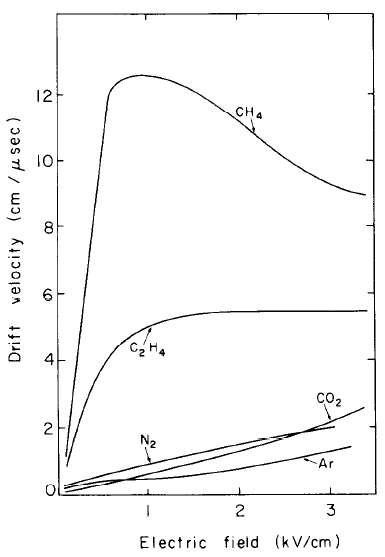
\includegraphics[width=6.7cm]{det05}
\end{floatingfigure}
\noindent
Средняя скорость движения электронов и ионов называется скоростью дрейфа,
её можно записать в виде: $v_d =\mu E$, где $\mu$ - подвижность ионов,
которая кроме напряжённости $Е$ в электрическом поле, зависит и от состава
газовой смеси, давления и температуры. На рисунке показана зависимость
скорости дрейфа электронов от напряжённости для некоторых смесей газа при
нормальных условиях.

Подвижность электронов в~газах приблизительно на три порядка больше чем
подвижность ионов.
% Ускорением ионов, электрическим полем, можно практически пренебречь.
Электроны, при достаточно большом значении напряжённости, смогут за
время между двумя столкновениями, приобрести в электрическом поле
энергию, достаточную для вторичной ионизации атомов газа, может произойти
газовое усиление. В результате число носителей зарядов возрастает.

%\subsubsection{Лавина электронов}
\subsubsection{Газовое усиление}
\begin{figure}[]\center
  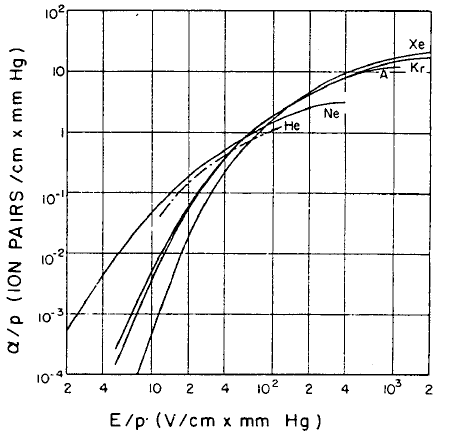
\includegraphics[scale=0.56]{det06}
  \caption{Первый коэффициент Таунсенда для разных инертных газов.}
  \label{fig:det06}
\end{figure}

При высоких значениях $E/p$, где $p$ - давление в газе, количество
вторичных электронов растёт лавинообразно. На рис.~\ref{fig:det06} видно,
что эффективное развитие лавины начинается в поле при $E/p \approx 100$
В/(см.мм рт.ст.) \cite{rop:04}.

Количество вторичных электронов в лавине $\alpha$\footnote{Зависимость
  $\alpha/p$ от $E/p$ (рис.~\ref{fig:det06}) можно описать эмпирическим
  выражением $\alpha/p = A~e^{-B(p/E)^k}$, где $A, B, k$ - константы газовых
  смесей.}, образованных одним электроном
на пути длины 1 см вдоль линии электрического поля,
называется первым коэффициентом Таунсенда, или коэффициентом ударной
ионизации. Если $N_0$ - число первичных электронов, созданных
ионизирующей
частицей, то полное число электронов $N(x)$ %собранных на аноде
в точке лавины~$x$ равно $N(x) = N_0~e^{\alpha x}$. Коэффициент газового
усиления можно определить как \cite{sau:02}:
\[
 u~=~\frac{N}{N_0}~=~e^ {\int \alpha(x) \,dx}.
%u~=~\frac{N}{N_0}~=~e^{\int\limits_0^{x{_0}} \alpha(x)\,dx}.
\]
Если использовать инертные (благородные) газы, можно получить эффект
газового усиления и при более низкой напряжённости электрического поля.
В таких газах электрон в основном теряет энергию на их ионизацию, а не на
возбуждение.

%\subsubsection{Однопроволочный пропорциональный счётчик}
\subsubsection{Режимы работы газовых детекторов}
Зависимость собравшихся ионов на электродах детектора --- регистрируемый
заряд от величины напряжённости электрического поля для газонаполненного
цилиндрического детектора показана на рис.~\ref{fig:det07} \cite{leo:94}.
\begin{figure}[h]\center
  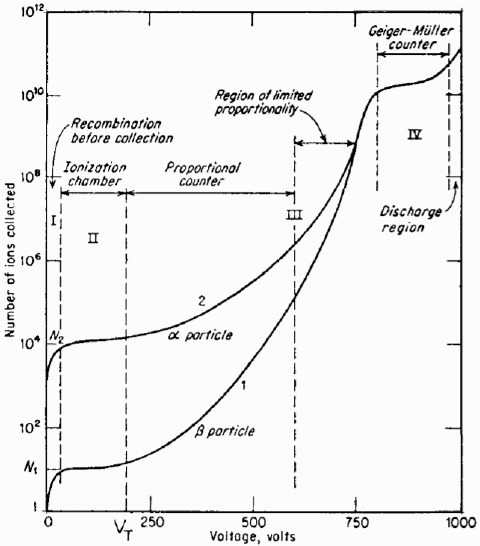
\includegraphics[width=10.8cm,height=11.2cm]{det07}
  \caption{Режимы работы газовых цилиндрических детекторов.}
  \label{fig:det07}
\end{figure}

В области напряжения I ионизации и собиранию заряда на электродах
препятствует процесс рекомбинации ионов. При увеличении напряжения
скорость ионов возрастает, рекомбинация уменьшается, амплитуда
возрастает.

В области II все образовавшейся ионы собираются на электродах. В этой
области работают ионизационные камеры.

При дальнейшем усилению напряжённости первоначальное число носителей
зарядов сильно возрастает, происходит газовое усиление. Участок III ---
область пропорционального режима. При более высоких электрических полях
образующийся заряд не будет зависит от первичной ионизации --- область
ограниченной пропорциональности.

В режиме работы счётчиков Гейгера-Мюллера, область IV,
% происходят огромные лавинообразный процесс,
регистрируемый сигнал становится одинаковым для частиц с различной
ионизацией (зависит только од напряжения). Регистрируется любая частица
способная создать хотя бы одну пару ионов в объёме счётчика.
%\subsubsection{Пропорциональный счётчик}

\subsection{Многопроволочные пропорциональные камеры}
Многопроволочная пропорциональная камера по сути представляет
набор цилиндрических пропорциональных счётчиков помешенных в одном
газовом объёме.
\begin{figure}[h]\center
  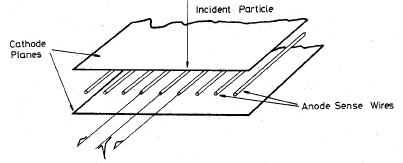
\includegraphics[scale=0.70]{det08}
  \caption{Схема конструкции многопроволочных пропорциональных камер.}
  \label{fig:det08}
\end{figure}
Схема такой камеры показана на рис.~\ref{fig:det08}. Между двумя
плоскими катодами из металлической фольги расположенные сигнальные
проволочки --- аноды (обычно это проволочки диаметром 20 мкм,
расположенные с шагом 2 мм).
\begin{figure}[h]\center
  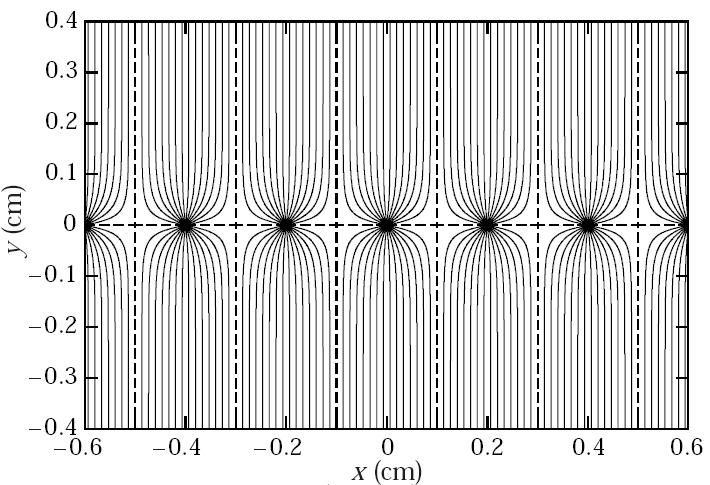
\includegraphics[width=10.8cm,height=6.2cm]{det09}
  \caption{Силовые линии электрического поля в пропорциональной камере
    с несколькими проволочками (симуляция программой GARFIELD \cite{gar}).}
  \label{fig:det09}
\end{figure}

Ионизирующая частица, проходящая через многопроволочную
пропорциональную камеру, образует вдоль своего пути свободные электроны,
которые зарождают лавины точно также, как и в пропорциональных счётчиках.
Заряд рождается в непосредственной близости от анодной проволочки
в области сильного электрического поля. Сигнал с каждой проволочки
регистрируется отдельно, что позволяет определить координату частицы
в камере.
\begin{figure}[h]\center
  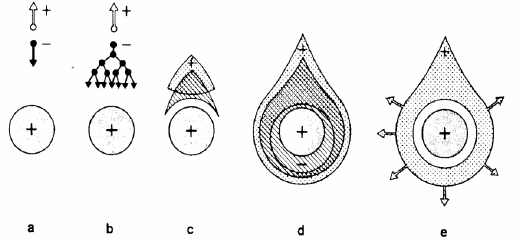
\includegraphics[width=12.0cm]{det10}
  \caption{Временно---пространственное развитие лавины вблизи анодной
    проволочки пропорциональной камеры.}
  \label{fig:det10}
\end{figure}

Поскольку большинство электронов рождается вблизи анода, они
проходят очень короткую область (несколько мкм) с малой разностью
потенциалов. Положительные ионы, дрейфующие в сторону катода, проходят
почти всю разность потенциалов. Это означает, что сигнал на анодной
проволочке создаётся, в основном, положительными ионами, а не
электронами \cite{pes:86}.

При конструкции многопроволочной пропорциональной камеры, желательно
чтобы диаметр анодной проволочки составлял приблизительно $1\%$ от
расстояния между ними, напряжённость электрического поля будет тогда
достаточной для газового усиления. В большинстве случаев в качестве анода
используются тонкие (диаметр от 10 до 30 мкм) вольфрамовые проволочки
гальванизированные золотом. Катодные плоскости обычно металлические
фольги или слои натянутых проволочек \cite{gru:99}.

При изготовлении камер, особенно больших размеров, электростатическое
отталкивание анодных проволочек приводит к проблеме их механической
нестабильности. Длинные проволочки нужно натягивать с большой силой, или
фиксировать на промежуточных расстояниях. Это в свою очередь приводит
к образованию локальных (неэффективных) зон в точке фиксации.

Пространственное разрешение камеры определяется в основном расстоянием
$d$ между проволочками. Среднеквадратичная ошибка вычисляется как
$\sigma = d/\sqrt 12$. Для типичного расстояния анодных проволок 2~мм,
погрешность определения координаты частицы, пересекающей камеру,
составляет $\sim 0.6$ мм. Уменьшение расстояния\footnote{Для получения
  нужного газового усиления, при уменьшении расстояния между
  проволочками, необходимо увеличивать напряжение.}
между анодными проволочками приводит к улучшению разрешения
% (кроме пространственного и временное).
Однако создание камер больших размеров с такими уменьшенными
межпроволочными расстояниями связано с рядом проблем, в том числе с
уже упомянутым электростатическим отталкиванием проволок.

Рабочие газы для пропорционального режима работы камеры должны иметь
высокий коэффициент газового усиления ---  инертные (благородные) газы.
В большинстве случаев используются аргон или ксенон с различными добавками,
в качестве которых чаще всего используются $CO_2, CH_4$, изобутан. С такими
смесями можно получить газовое усиление $\sim 10^5$ а эффективность
регистрации частицы близкая $100\%$. Использование так называемой
магической смеси ($75\%~Ar + 24.5\%~изобутана + 0.5\%~фреона$) позволяет
увеличить коэффициент газового усиления до $\sim 10^8$ \cite{zan:78}.

\subsection{Дрейфовые камеры}
Идея определения координаты частицы, вызывающей ионизацию газа,
измерением времени дрейфа первичных электронов в однородном
электрическом поле, была высказана уже вскоре после\footnote{
  Пропорциональные многопроволочные и дрейфовые камеры появились
  в 1968 году. Ж. Шарпак за вклад в открытие и создание детекторов
  получил в 1992 году Нобелевскую премию.}
появления многопроволочной пропорциональной камеры \cite{char:93}.

Разница во времени $\delta t$ определяется между моментом первичной
ионизации (прохождением частицы) $t_0$ и моментом, когда электроны
достигают анодной проволочки (попаданием облака заряда) $t_1$. Координату
$x$ места прохождения частицы можно вычислить с помощью следующего
выражения:
\[
x=\int_{t_0}^{t_1} v_d(t)\,\delta t
\]

Желательную постоянную скорость дрейфа $v_{d}$ можно достичь
образованием постоянной напряжённости электрического поля вдоль пути
дрейфующего электрона.
%Длина этой пути может достигать и несколько десятков сантиметров.
Между соседними анодными проволочками (находящимися под потенциалом
+ HV 2) вводятся дополнительные, потенциальные проволочки под
потенциалом - HV 1. На катодные проволочки подан распределённый
потенциал от 0 до - HV 1, рис.~\ref{fig:det11} \cite{sau:77}.
\begin{figure}[h]\center
  \hspace*{-0.2cm}
  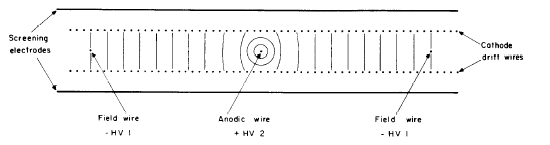
\includegraphics[scale=0.75]{det11}
  \caption{Схематический вид ячейки дрейфовой камеры с проволочными
    катодами.}
  \label{fig:det11}
\end{figure}

Пространственное разрешение дрейфовых камер определяется однородностью
электрического поля в области дрейфа. Как видно из рис.~\ref{fig:det12}
ограничение в разрешение вносит ещё временное разрешение электроники,
\begin{figure}[h]\center
  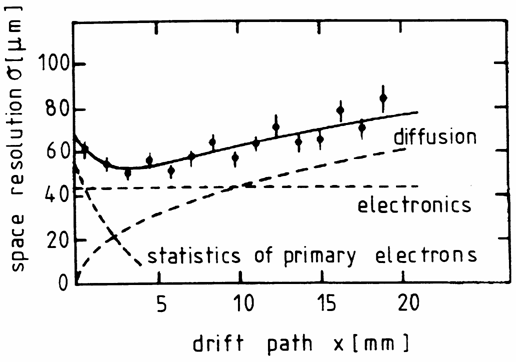
\includegraphics[scale=1.00]{det12}
  \caption{Зависимость пространственного разрешения дрейфовой камеры
    от пути дрейфа.}
  \label{fig:det12}
\end{figure}
диффузия электронов во время их дрейфа к аноду и статистическая
флуктуация первичной ионизации в близости анодной проволочки. Заметим,
что для частиц, проходящих под наклоном к плоскости камеры, разрешение
ухудшается (для очень больших наклонов почти в два раза).

\clearpage
\thispagestyle{plain}
\section{Заключение}
В представленном обзоре отражены лишь основные характеристики работы
газонаполненных координатно-трековых детекторов. Он не претендует на
полноту и не преследует цель охватить все развитые модификации
рассматриваемых устройств.

Упор сделан на пояснение принципов работы и происходящие физические
процессы при формировании сигналов от проходящих заряженных частиц.
В связи с этим в первой части обзора уделено внимание взаимодействию
частиц с веществом. Дана короткая информация о различных трековых приборах,
с их преимущества и недостатки с целью подчеркнуть ту нишу в детектировании
частиц, которая принадлежит газовым трековым детекторам.

\clearpage
\thispagestyle{empty}
\begin{landscape}
  \vspace*{1.3cm}
  \hspace*{-1.0cm}
  \large
  \begin{tabular}[c]{|p{6.0cm}|p{2.0cm}|p{1.8cm}|p{5.0cm}|p{5.0cm}|}
    \hline
    Трековый детектор & разреше\-ние [мкм] & мёртвое время [мс] &
    преимущества & недостатки
    \tabularnewline
    \hline
    \hline
    \slshape Камера Вильсона & 300 & $10^5$ & простота, первый трековый
    детектор & большое мёртвое время
    \tabularnewline
    \hline
    \slshape Пузырьковая камера & 20 & $10^2$ & анализ сложных
    событий & неуправляемость
    \tabularnewline
    \hline
    \slshape Искровая камера & 200 & $10$ & простота конструкции
    & низкая многотрековая эффективность
    \tabularnewline
    \hline
    \slshape Ядерная фотоэмульсия & 5 & 0 & пространственное
    разрешение, цена & трудоёмкий анализ событий
    \tabularnewline
    \hline
    \slshape Пропорциональные камеры & 200 & $10^-5$ & временное
    разрешение, простота & механическая нестабильность проволочек
    \tabularnewline
    \hline
    \slshape Дрейфовая камера & 50 & $10^-4$ & координатное
    разрешение & зависимость разрешения от диффузии и первичной
    ионизации
    \tabularnewline
    \hline
  \end{tabular}
\end{landscape}



%%% Local Variables:
%%% TeX-master: "referat"
%%% End:


\clearpage
\pagestyle{plain}
\begin{thebibliography}{99}
  % \bibitem{pom:84}
  %   \emph{Померанчук И. //} Название журнала. - Год выпуска. - Номер
  %   выпуска. - Местоположение статьи (страницы).

\bibitem{pdg}
  \emph{W. Yao et al. //} Journal of Physics G 33, 2006, \\
  available on the pages http://pdg.lbl.gov

\bibitem{cer:04}
  \emph{А. Черняев //} Взаимодействие ионизирующего излучения с веществом,
  2004, Физматлит

\bibitem{kor:06}
  \emph{A. Korytov //} Interactions of particles with matter, 2006, \\
  http://www.phys.ufl.edu/\textasciitilde korytov/phz5354/
  note\_C09\_interaction\_of\_particles\_with\_matter.pdf

\bibitem{sta}
  \emph{S. Stapnes //} Instrumentation for high-energy physics, \\
  http://www.fys.uio.no/\textasciitilde stapnes/pylos-I.doc

\bibitem{den:04}
  \emph{П. Денисов //} Детекторы черенковского излучения, 2004, Природа

\bibitem{mas:06}
  \emph{F. Maas //} Interaction of Particles with Matter and Main Types
  of Detectors, 2006, \\
  http://www.fantom.kvi.nl/edact.html

\bibitem{kal:66}
  \emph{В. Калашникова //} Детекторы элементарных частиц, 1966, Наука

\bibitem{shut:66}
  \emph{R. Shutt //} High enrgy physics with the Brokhaven 80'' hydrogen buble
  chamber, 1996, \\  http://www.bnl.gov/bnlweb/PDF/bnl\_9065.pdf

\bibitem{har}
  \emph{G. Harigel //} Bubble chambers, technology and impact on high enrgy
  physics, \\ http://dbserv.ihep.su/~pubs/aconf00/tconf00/ps/c6-4.pdf

\bibitem{gla}
  \emph{В. Глаголев //} 100-см водородная пузырьковая камера, k 50-летию ЛВЭ

\bibitem{duk:04}
  \emph{C. Dukes //} Spark Chambers for the Finesse Rangestack, 2004,
  \\ http://galileo.phys.virginia.edu/research/groups/hep/aag/memos/
  spark\_chamber.pdf

\bibitem{nak:06}
  \emph{T. Nakamura et al. //} Nucl. Instr. and Meth. A, 2006, Vol. 556,
  p.~80-86

\bibitem{kla:90}
  \emph{К. Клайнкнехт //} Детекторы корпускулярных излучений, 1990, Мир

\bibitem{rop:04}
  \emph{L. Ropelewski et al. //} CERN Academic Training Programme 2004/2005,
  Lecture 2a - Gas Detectors, \\
  http://ph-dep-dt2.web.cern.ch/ph-dep-dt2/CAT2005\_2a.pdf

\bibitem{sau:02}
  \emph{F. Sauli //} Gas-filled detectors, Short Courses-2002-1,\\
  http://fabio.home.cern.ch/fabio/seminars.res/ieee02\_sc\_sauli1.pdf

\bibitem{leo:94}
  \emph{W. Leo //} Techniques for nuclear and particle physics experiments,
  1994, Springer-Verlag

\bibitem{gar}
  \emph{R. Veenhof //} Garfield - simulation of gaseous detectors,
  CERN Program Library W5050, \\ http://garfield.web.cern.ch/garfield

\bibitem{pes:86}
  \emph{В. Пешехонов //} Физ. элем. частиц и атом. ядра, 1986, Т. 17,
  \No 5, с.~1030-1078

\bibitem{gru:99}
  \emph{К. Групен //} Детекторы элементарных частиц, 1999, Сибирский
  хронограф

\bibitem{zan:78}
  \emph{Ю. Заневский //} Проволочные детекторы элементарных частиц,
  1978, Атомиздат

\bibitem{char:93}
  \emph{Ж. Шарпак //} Успехи физических наук, 1993, T. 163, \No 10, \\
  с.~57-66

\bibitem{sau:77}
  \emph{F. Sauli //} CERN Academic Training Programme 1975/1976,
  Principles of operation of multiwire proportional and drift chambers
\end{thebibliography}

\end{document}



%%% Local Variables:
%%% TeX-master: t
%%% End:
